
%-=-=-=-=-=-=-=-=-=-=-=-=-=-=-=-=-=-=-=-=-=-=-=-=
%
%        LOADING DOCUMENT
%
%-=-=-=-=-=-=-=-=-=-=-=-=-=-=-=-=-=-=-=-=-=-=-=-=

\documentclass[compress]{beamer}
\usetheme{sthlm}

%-=-=-=-=-=-=-=-=-=-=-=-=-=-=-=-=-=-=-=-=-=-=-=-=
%        LOADING BEAMER PACKAGES
%-=-=-=-=-=-=-=-=-=-=-=-=-=-=-=-=-=-=-=-=-=-=-=-=

\usepackage{
booktabs,
datetime,
dtklogos,
graphicx,
multicol,
pgfplots,
ragged2e,
tabularx,
tikz,
wasysym
}

\pgfplotsset{compat=1.8}
\usepackage[T1]{fontenc}
\usepackage{newpxtext,newpxmath}
\usepackage{pifont}% http://ctan.org/pkg/pifont
\usepackage[utf8x]{inputenc}
\usepackage{pgfpages}
\usepackage{multicol}
\usepackage{caption}
\usepackage{pgfgantt}
\usepackage{graphicx} % Allows including images
\usepackage{booktabs} % Allows the use of \toprule, \midrule and \bottomrule in tables
\usepackage{listings}
\usepackage{color, colortbl}

\definecolor{mygreen}{HTML}{4cd964}
\newcommand{\cmark}{{\color{mygreen}\ding{51}}}%
\newcommand{\xmark}{{\color{red}\ding{55}}}%


%\setbeameroption{show notes on second screen=right}


\lstset{ %
language=[LaTeX]TeX,
basicstyle=\normalsize\ttfamily,
keywordstyle=,
numbers=left,
numberstyle=\tiny\ttfamily,
stepnumber=1,
showspaces=false,
showstringspaces=false,
showtabs=false,
breaklines=true,
frame=tb,
framerule=0.5pt,
tabsize=4,
framexleftmargin=0.5em,
framexrightmargin=0.5em,
xleftmargin=0.5em,
xrightmargin=0.5em
}

%-=-=-=-=-=-=-=-=-=-=-=-=-=-=-=-=-=-=-=-=-=-=-=-=
%        LOADING TIKZ LIBRARIES
%-=-=-=-=-=-=-=-=-=-=-=-=-=-=-=-=-=-=-=-=-=-=-=-=

\usetikzlibrary{
backgrounds,
mindmap
}

%-=-=-=-=-=-=-=-=-=-=-=-=-=-=-=-=-=-=-=-=-=-=-=-=
%        BEAMER OPTIONS
%-=-=-=-=-=-=-=-=-=-=-=-=-=-=-=-=-=-=-=-=-=-=-=-=

%\setbeameroption{show notes}

%-=-=-=-=-=-=-=-=-=-=-=-=-=-=-=-=-=-=-=-=-=-=-=-=
%        BEAMER COMMANDS
%-=-=-=-=-=-=-=-=-=-=-=-=-=-=-=-=-=-=-=-=-=-=-=-=


%-=-=-=-=-=-=-=-=-=-=-=-=-=-=-=-=-=-=-=-=-=-=-=-=
%
%	PRESENTATION INFORMATION
%
%-=-=-=-=-=-=-=-=-=-=-=-=-=-=-=-=-=-=-=-=-=-=-=-=
\usepackage{tikz}
\usepackage{pgf}

\newcommand\Wider[2][3em]{%
\makebox[\linewidth][c]{%
  \begin{minipage}{\dimexpr\textwidth+#1\relax}
  \raggedright#2
  \end{minipage}%
  }%
}

\logo{
\includegraphics[height=1.5cm]{logo.pdf}}
\newcommand{\nologo}{\setbeamertemplate{logo}{}}
\definecolor{Gray}{gray}{0.9}
\newcommand{\myquote}[2]{\begin{exampleblock}{}{\large ``#1''}\vskip5mm\hspace*\fill{\small--- #2}\end{exampleblock}}
%----------------------------------------------------------------------------------------
%	TITLE PAGE
%----------------------------------------------------------------------------------------

\title{Hyper-linked Communications} 
\subtitle{WebRTC enabled asynchronous collaboration}


\author{Henrique Rocha} % Your name
\institute[IST] % Your institution as it will appear on the bottom of every slide, may be shorthand to save space
{
Instituto Superior Técnico \\
Universidade de Lisboa \\ % Your institution for the title page
\medskip
\textit{henrique.rocha@tecnico.ulisboa.pt}\\ % Your email address
\small

Supervisors: Ricardo Pereira \& Paulo Chainho
}
\date{\today} % Date, can be changed to a custom date

\begin{document}
{
\nologo
\begin{frame}
\maketitle % Print the title page as the first slide

\note{Boa Tarde! \\ Comunicações hiperligadas - Colaboração através de WebRTC}
\end{frame}
}

\begin{frame}[t]
\frametitle{Overview} 
\tableofcontents[hidesubsections]
\note{Introdução, Estado de arte\\
Arquitectura, implementação e avaliação da nossa proposta\\
Por fim as conlusões e trabalhos futuro}


\end{frame}

%----------------------------------------------------------------------------------------
%	PRESENTATION SLIDES
%----------------------------------------------------------------------------------------

%------------------------------------------------

\section{Introduction}\label{intro}

%\begin{frame}[t,shrink]
%\frametitle{Introduction} 
%\tableofcontents[currentsection,hideothersubsections]
%\end{frame}

	\subsection{Context}   % English
		\begin{frame}[c]
		\frametitle{Context}
		Written communication could never replace face to face communication.

		\myquote{No computer in our lifetimes will ever rival a human voice's capacity to conveying rich and complex social and emotional meaning}{Geddes, Martin}

		Today, we can achieve more.
		\end{frame}

	\subsection{Problem Statement} % English
  		\begin{frame}[c]
		\frametitle{Problem Statement}
		
		An application that provides a collaborative environment and a way to remember our past communications would be a strong tool.
		
		\vfill

		Real-time communication applications can make a difference on business, education and health sectors.

		\end{frame}






		
	

	\subsection{Thesis Goals} % English
  		\begin{frame}[c]
		\frametitle{Thesis Goals}
		Allow multi party conference calls.

		\vfill
		
		Record and playback interactive video.
		
		\vfill

        Create a collaborative environment        

        \vfill

		Use only standard technologies like JavaScript, WebRTC, HTML5 and CSS3.


		\end{frame}


\section{Related Work}\label{related}

%\begin{frame}[t,shrink]
%\frametitle{Related Work} 
%\tableofcontents[currentsection,hideothersubsections]
%\end{frame}
	\begin{frame}[c]
			\frametitle{State of the Art overview}
	\begin{enumerate}
		\item Connection Establishment
		\item Streaming audio and video
		\item Overlay communications with content
		\item Collaboration Environment
	\end{enumerate}


	\end{frame}

  		\begin{frame}[c]
		\frametitle{Connection Establishment}
		\begin{itemize}
	%	\item IPv4 Address Exhaustion
	%	\vfill
		\item Network Address Translation	
		\vfill
		%\item Client-Server model
		%--\vfill
		\item STUN + TURN = ICE
		\end{itemize}
		\begin{flushright}

			\vspace*{-4\baselineskip}
			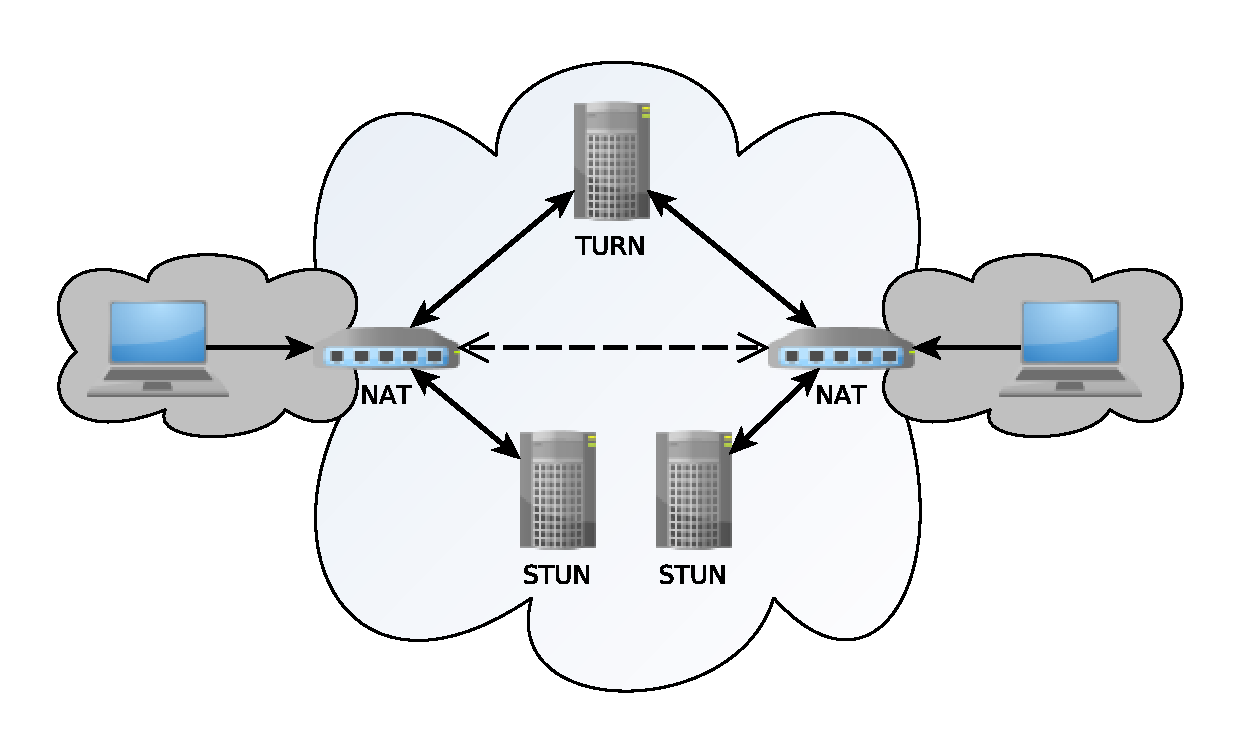
\includegraphics[width=0.55\textwidth]{figures/ice.pdf}
		\end{flushright}
		
		\end{frame}

		\begin{frame}[c]
		\frametitle{Streaming audio and video}

		WebRTC (Web Real-Time Communications)

		\begin{itemize}
		\item Access to camera, microphone and screen*
		\item Peer to Peer file and stream sharing
		\item Standardized protocols
		\item No plug-ins required
		\end{itemize}

		\begin{flushright}

			\vspace*{-5\baselineskip}
			
\includegraphics[width=0.2\textwidth]{figures/webrtc.png}
		\end{flushright}
		
			\tiny{* requires installing a plug-in yet.}

		\end{frame}

  		\begin{frame}[c]
		\frametitle{Overlay communications with content}
		\begin{itemize}
		\item \textbf{Concepts:} HyperMedia \& Detail on Demand
		\vfill
		\item \textbf{Implementations:} HyperCafe \& HyperHitchcock  % Detail on Demand
				
		\end{itemize}
		
		\begin{figure}
			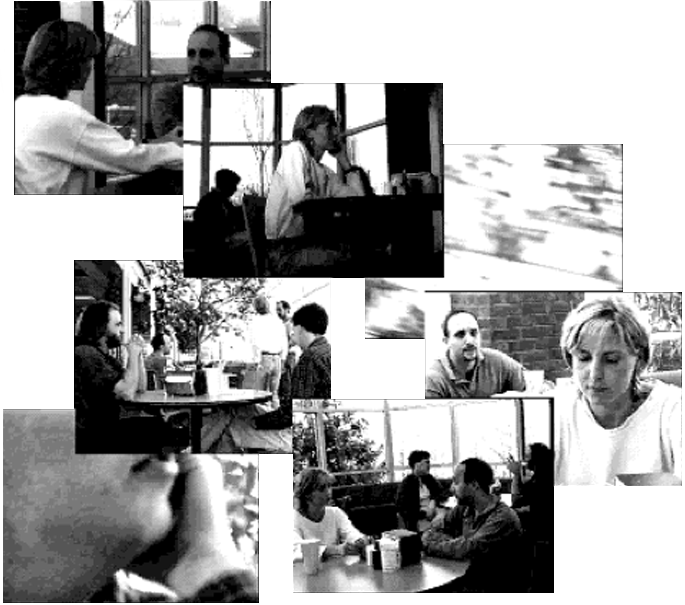
\includegraphics[height=0.4\textheight]{figures/hypercafe.png}
			
\includegraphics[height=0.1\textheight]{figures/space.png}
			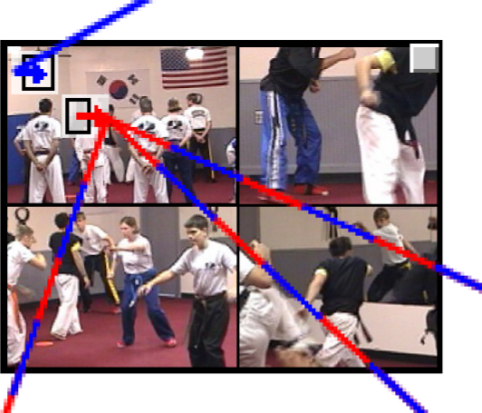
\includegraphics[height=0.4\textheight]{figures/hitchcock.png}
		\end{figure}
		\end{frame}


%		\begin{frame}[c]
%		\frametitle{Hypermedia: more than words, more than images}
%		\begin{itemize}		
%		\item \textbf{Languages:} HyVAL \& SMIL
%		\vfill
%		\item \textbf{WebBrowser:} Ambulant \& SmillingWeb \& SVG
%		\end{itemize}
%		
%		\begin{multicols}{2}
%		\begin{figure}
%			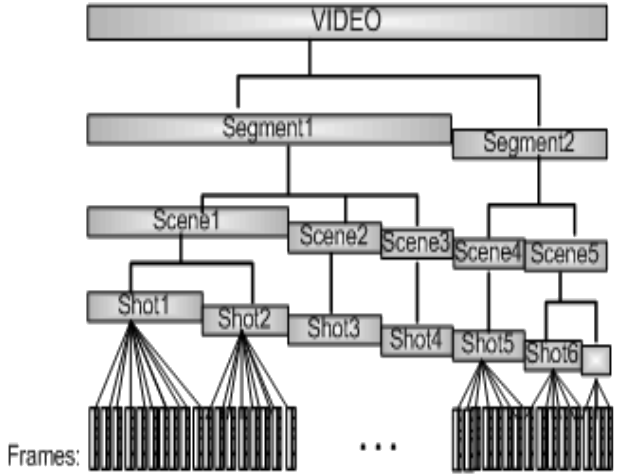
\includegraphics[height=0.4\textheight]{figures/hyval.png}
%			\caption{HyVAL structure}
%		\end{figure}
%		\begin{figure}
%			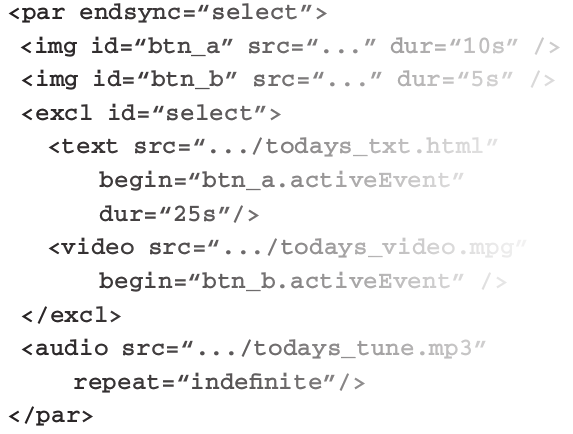
\includegraphics[height=0.4\textheight]{figures/smil.png}
%			\caption{SMIL example}
%		\end{figure}
%		\end{multicols}
%		\end{frame}


% 		\begin{frame}[c]
%		\frametitle{Web-Browser plug-ins}
%		\begin{figure}
%			
\includegraphics[height=0.3\textheight]{figures/flash.jpg}
%			
\includegraphics[height=0.1\textheight]{figures/space.png}
%			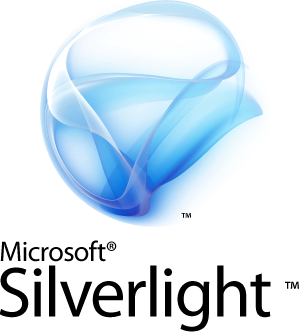
\includegraphics[height=0.3\textheight]{figures/silverlight.png}
%		\end{figure}
%		\end{frame}


% 		\begin{frame}[c]
%		\frametitle{Extending collaboration tools with time manipulation}
%	
%		\begin{figure}
%			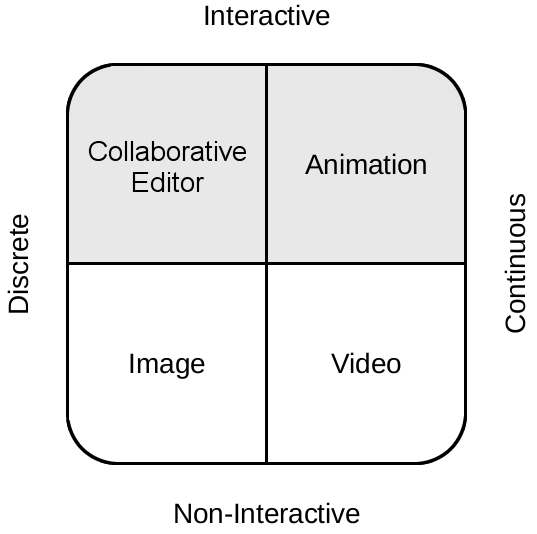
\includegraphics[height=0.5\textheight]{figures/media_types.png}
%			\caption{Media Types}
%		\end{figure}
%		\end{frame}



  		\begin{frame}[c]
		\frametitle{Collaboration Environment}

			\begin{table}
			\centering
			\caption{Comparison between Operational Transformation libraries}
			\label{table:otcomparision}
			\begin{tabular}{|c|c|c|c|}
			\hline
			\textbf{Library} & \textbf{Server Freedom} & \textbf{Storage Freedom} & \textbf{Operations} \\ \hline
			ShareJS          & \xmark                 & \xmark                  & text+objects        \\ \hline
			TogetherJS       & \xmark                 & \cmark                   & text+objects        \\ \hline
			Goodow           & \xmark                 & \xmark                  & text+objects        \\ \hline
			Etherpad Lite    & \xmark                 & \xmark                  & extendable 			    \\ \hline
			OT.js            & \cmark                  & \cmark                   & text                \\ \hline
			\end{tabular}
			\end{table}

		\end{frame}

	\subsection{Overview}


		\begin{frame}[c]
		\frametitle{Overview}

\begin{table}[]
\centering
%\caption{My caption}
\label{my-label}
	\resizebox{\textwidth}{!}{%

\begin{tabular}{rcccccc} 
  &
 \begin{minipage}{.1\textwidth}
\includegraphics[width=\linewidth]{figures/skype.png}\end{minipage} &  
 \begin{minipage}{.1\textwidth}
\includegraphics[width=\linewidth]{figures/hangouts.png}\end{minipage} &  
 \begin{minipage}{.1\textwidth}
\includegraphics[width=\linewidth]{figures/jitsi.png}\end{minipage} &  
 \begin{minipage}{.1\textwidth}
\includegraphics[width=\linewidth]{figures/kurento.png}\end{minipage} 
 &
 \begin{minipage}{.1\textwidth}
\includegraphics[width=\linewidth]{figures/logo.png}\end{minipage} \\

\tiny Name & \tiny Skype & \tiny Hangouts & \tiny Jitsi & \tiny Kurento & \tiny Our proposal   \\
\tiny Technology & \tiny Proprietary & \tiny WebRTC$^{1}$ & \tiny WebRTC & \tiny WebRTC & \tiny WebRTC \\
\tiny Development & \xmark & \cmark \tiny $^2$ & \cmark & \cmark & \cmark \\
\tiny Audio/Video & \cmark & \cmark & \cmark & \cmark & \cmark \\
\tiny Text Messaging & \cmark & \cmark & \cmark & \xmark  & \cmark \\
\tiny Collaborative Editor & \xmark & \cmark & \cmark & \xmark  & \cmark \\
\tiny File sharing & \cmark & \cmark & \cmark & \xmark  & \cmark\\
\tiny Recording \& Playback  & \xmark & \xmark & \xmark & \cmark  & \cmark \\
\tiny Interactive Content  & \xmark & \xmark & \xmark & \xmark  & \cmark 


\end{tabular}}
\end{table}

	\tiny{$^1$ requires installing a plug-in on non chrome web browsers.}

	\tiny{$^2$ allows the development of extensions.}

		\end{frame}




%	\subsection{Signaling}
%  		\begin{frame}[c]
%		\frametitle{Signaling: meet and get to know}
%		\begin{itemize}
%		\item Own Implementation
%		\vfill
%		\item SIP
%		\vfill
%		\item XMPP
%		\vfill
%		\item SigOFly 
%		\end{itemize}
%		\end{frame}



%\subsubsection{Streaming and Recording}\label{recstream}
%\subsubsection{Media Types}\label{mediatype}
%\subsubsection{Recording and Streaming Interactive Media}\label{intrecord}
%\subsubsection{Collaborative Environment}\label{collabenv}



\section{Architecture}\label{arch}

%\begin{frame}[t,shrink]
%\frametitle{Related Work} 
%\tableofcontents[currentsection,hideothersubsections]
%\end{frame}

\subsection{Modules}

	\begin{frame}[c]
		\frametitle{Modules}
		\begin{figure}[H]
			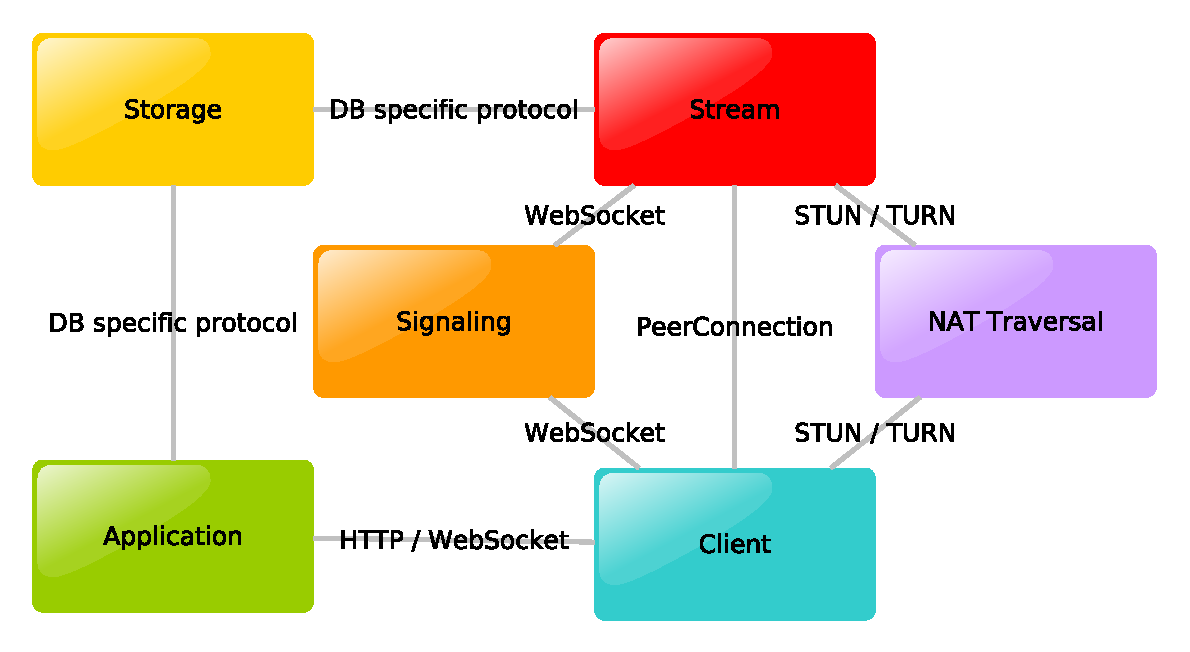
\includegraphics[width=0.8\textwidth]{figures/modules.pdf}
		\end{figure}
	\end{frame}

\subsection{Implementation Proposal}

		\begin{frame}[c]
		\frametitle{System Infrastructure}
		\begin{figure}[H]
			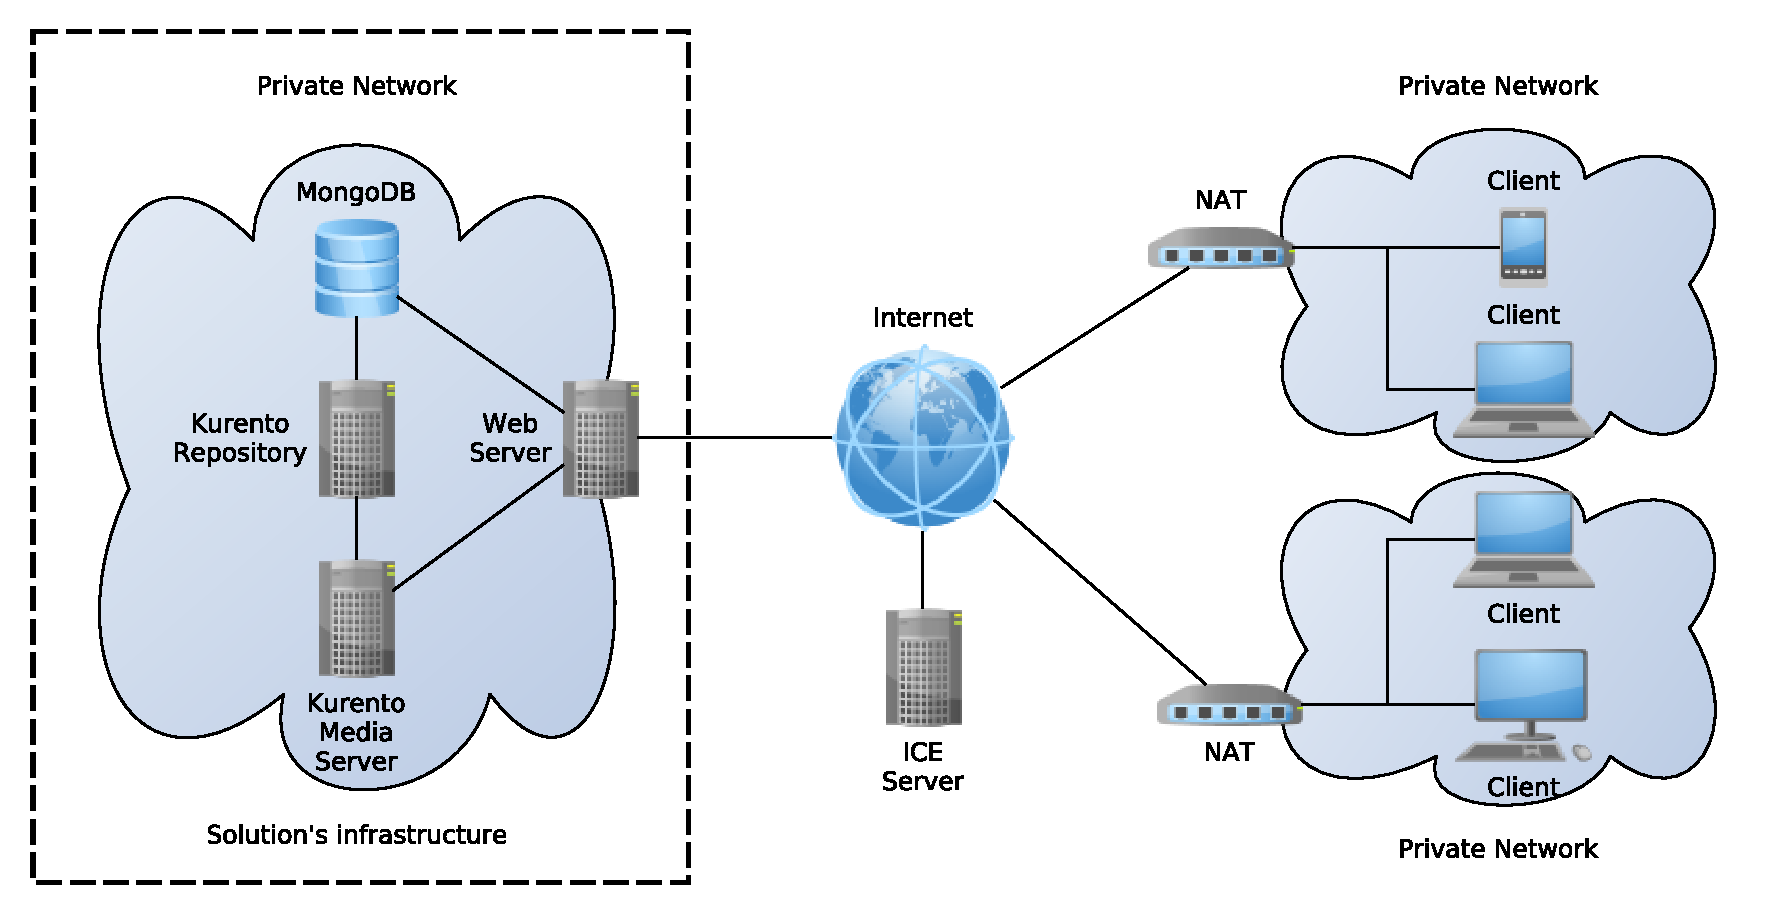
\includegraphics[width=0.9\textwidth]{figures/infrastructure.pdf}
		\end{figure}
		\begin{itemize}
		\scriptsize \item \textbf{Signaling Server \& Web Server}: Play Framework
		\scriptsize \item \textbf{Stream Server}: Kurento Media Server		
		\scriptsize \item \textbf{Storage}: MongoDB \& Kurento Repository
		\scriptsize \item \textbf{NAT Traversal}: Public STUN Servers
		\end{itemize}




		\end{frame}

		\begin{frame}[c]


		\frametitle{Application Architecture}

\Wider{
			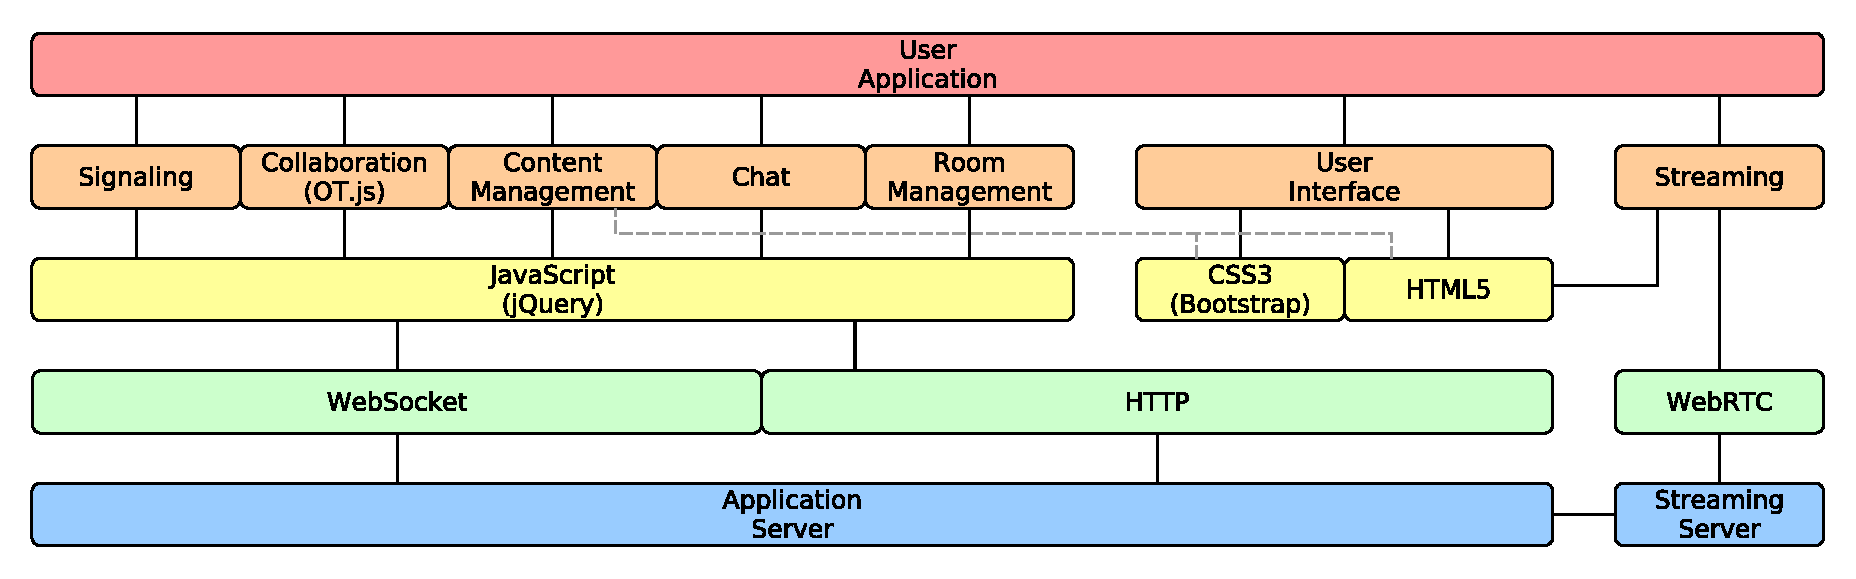
\includegraphics[width=\textwidth]{figures/app.pdf}

}

		\end{frame}


\section{Implementation}\label{meth} % Section
%\begin{frame}[t,shrink]
%\frametitle{Implementation} 
%\tableofcontents[currentsection,hideothersubsections]
%\end{frame}

\subsection{Signaling Protocol}
\begin{frame}[c]
		\frametitle{Signaling Protocol - Part 1}
		\begin{figure}[H]
			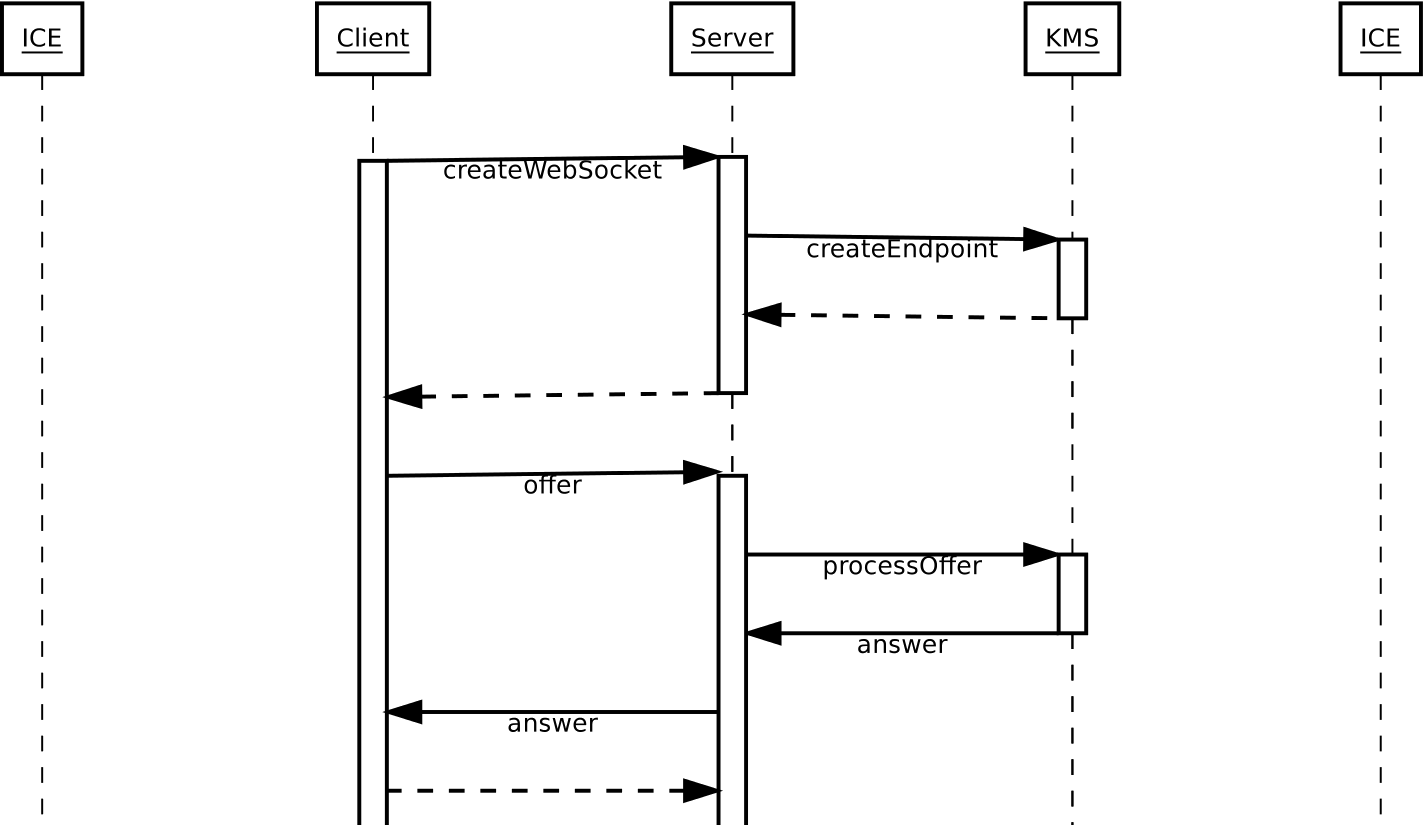
\includegraphics[width=0.9\textwidth]{figures/signaling1.png}
		\end{figure}
\end{frame}
\begin{frame}[c]
		\frametitle{Signaling Protocol - Part 2}
		\begin{figure}[H]
			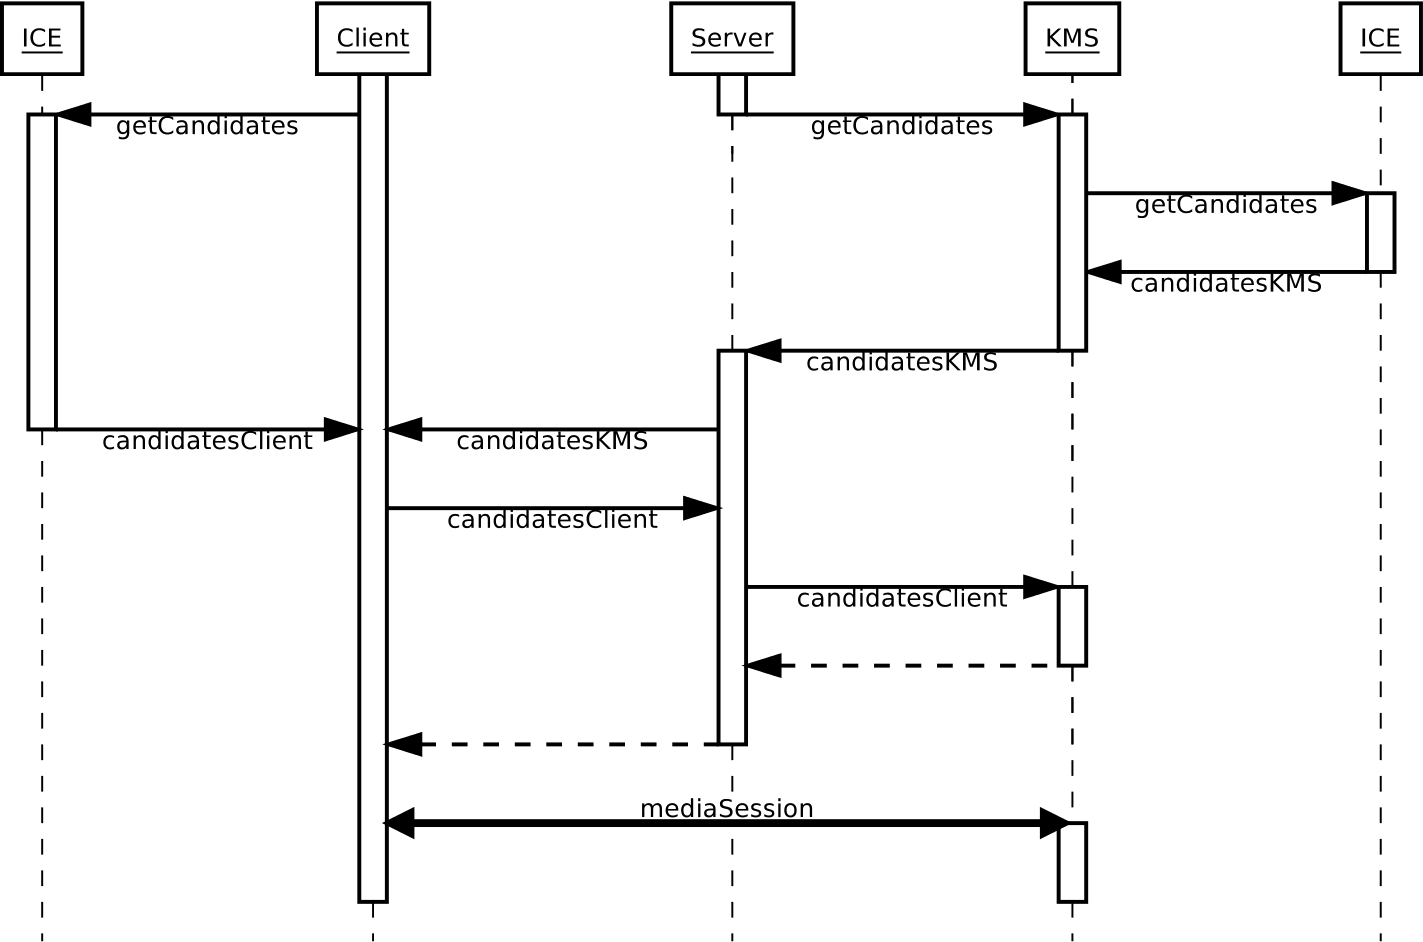
\includegraphics[width=0.9\textwidth]{figures/signaling2.png}
		\end{figure}
\end{frame}


\subsection{Stream operations}
	\begin{frame}[c]
		\frametitle{Stream operations}

		\begin{itemize}
			\item Server-side recording to database (Kurento Repository).
			\item Server-side stream composition.
			\item Speech detection.
		\end{itemize}
		\begin{figure}
			\vspace*{-1.5\baselineskip}

			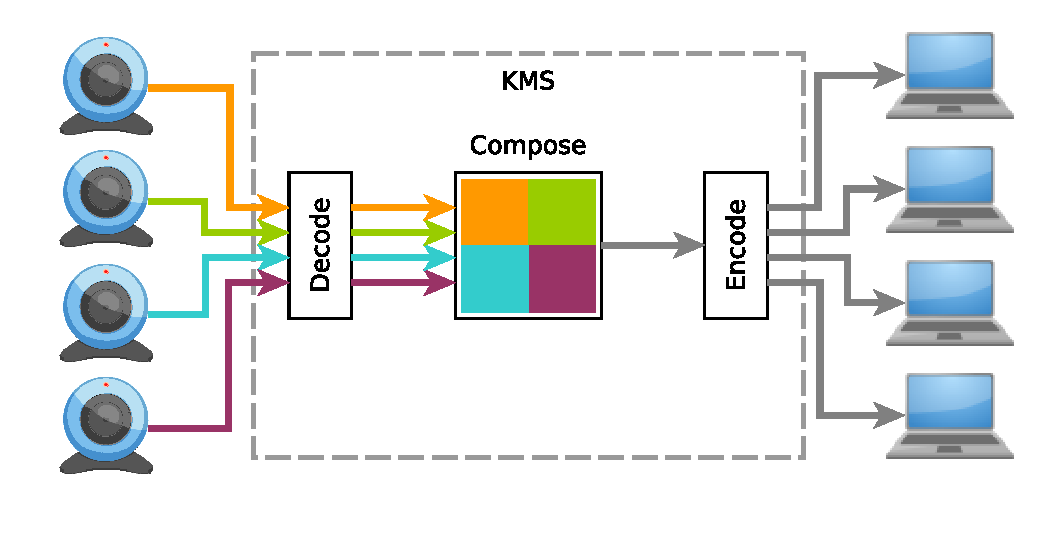
\includegraphics[width=0.6\textwidth]{figures/wcomposite.pdf}
			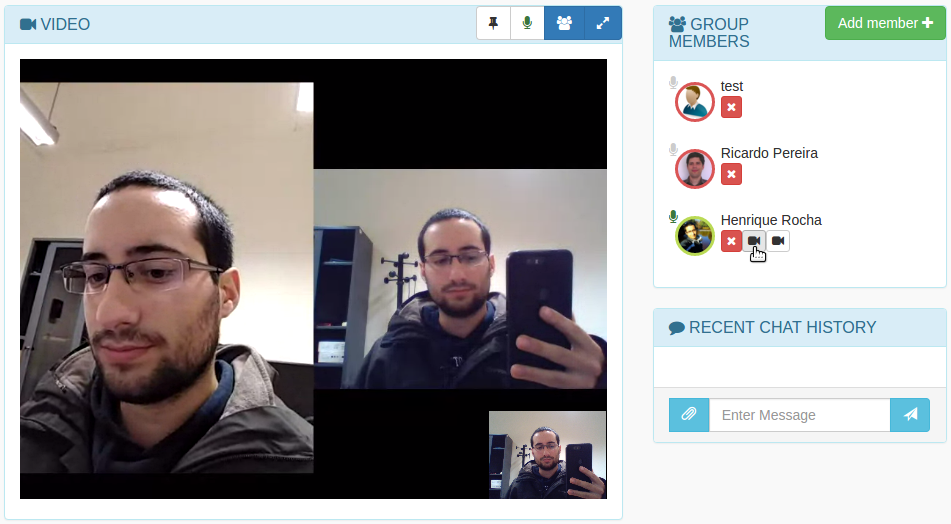
\includegraphics[width=0.4\textwidth]{figures/devices.png}
		\end{figure}
		\end{frame}


\subsection{Hyper-Content}

		\begin{frame}[c]
		\frametitle{Hyper-Content}


		\begin{itemize}
			\item Create \& Search content \vfill
			\item Scheduler \vfill
			\item QR codes \vfill
			\item Security concerns
		\end{itemize}

		\begin{flushright}

			\vspace*{-11\baselineskip}
			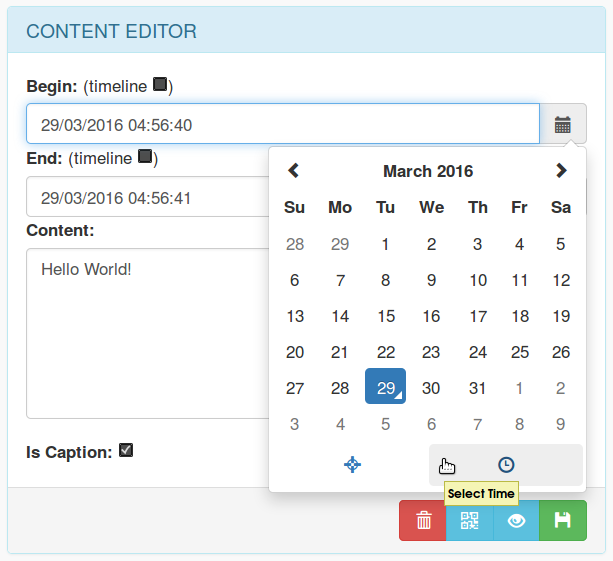
\includegraphics[width=0.5\textwidth]{figures/edition.png}
		\end{flushright}
		

		\end{frame}


\subsection{Time manipulation}

		\begin{frame}[c]
		\frametitle{Time manipulation}


		\begin{itemize}
		\item Playback recordings
		\vfill
		\item Create time hyper-links \& annotations
		\vfill
		\item Search annotations \& content
		\vfill
		\end{itemize}

		%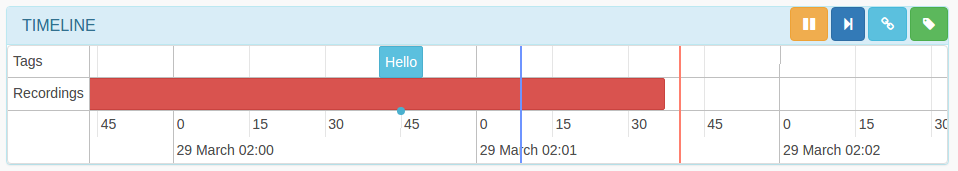
\includegraphics[width=\textwidth]{figures/timeline.png}
		%\begin{flushright}
		%\vspace*{-12\baselineskip}
		%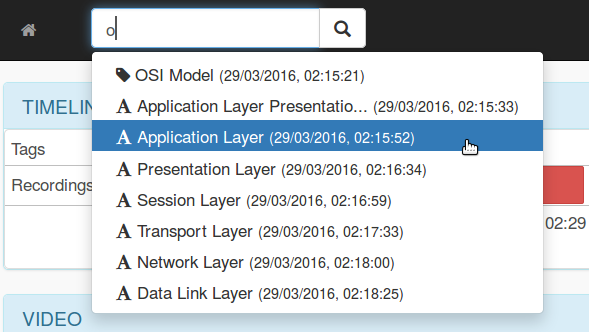
\includegraphics[width=0.45\textwidth]{figures/search.png}
		%\end{flushright}
		

		\end{frame}


\subsection{Chat \& Collaborative environment}

		\begin{frame}[c]
		\frametitle{Chat \& Collaborative environment}


		\begin{itemize}
		\item Instant text messaging
			\begin{itemize}
			\item WebSockets
			\end{itemize}

		\item File sharing
			\begin{itemize}
			\item HTTP file upload
			\item stored in the database
			\end{itemize}
		
		\item Collaborative text editor (OT.js)
			\begin{itemize}
			\item retain
			\item insert
			\item delete
			\end{itemize}
		

		\end{itemize}
		

		\end{frame}

  		\begin{frame}[c]
		\frametitle{Demonstration}
		%A teacher record and streams an interactive class, some students participate in real-time others may participate later.
		%\vfill
		%The teacher adds information to its class (create tags, add links, overlay images ...).
		%\vfill
		%Students can answer to quizzes.
	
		\begin{center}
		%\href{run:video.mkv}{
		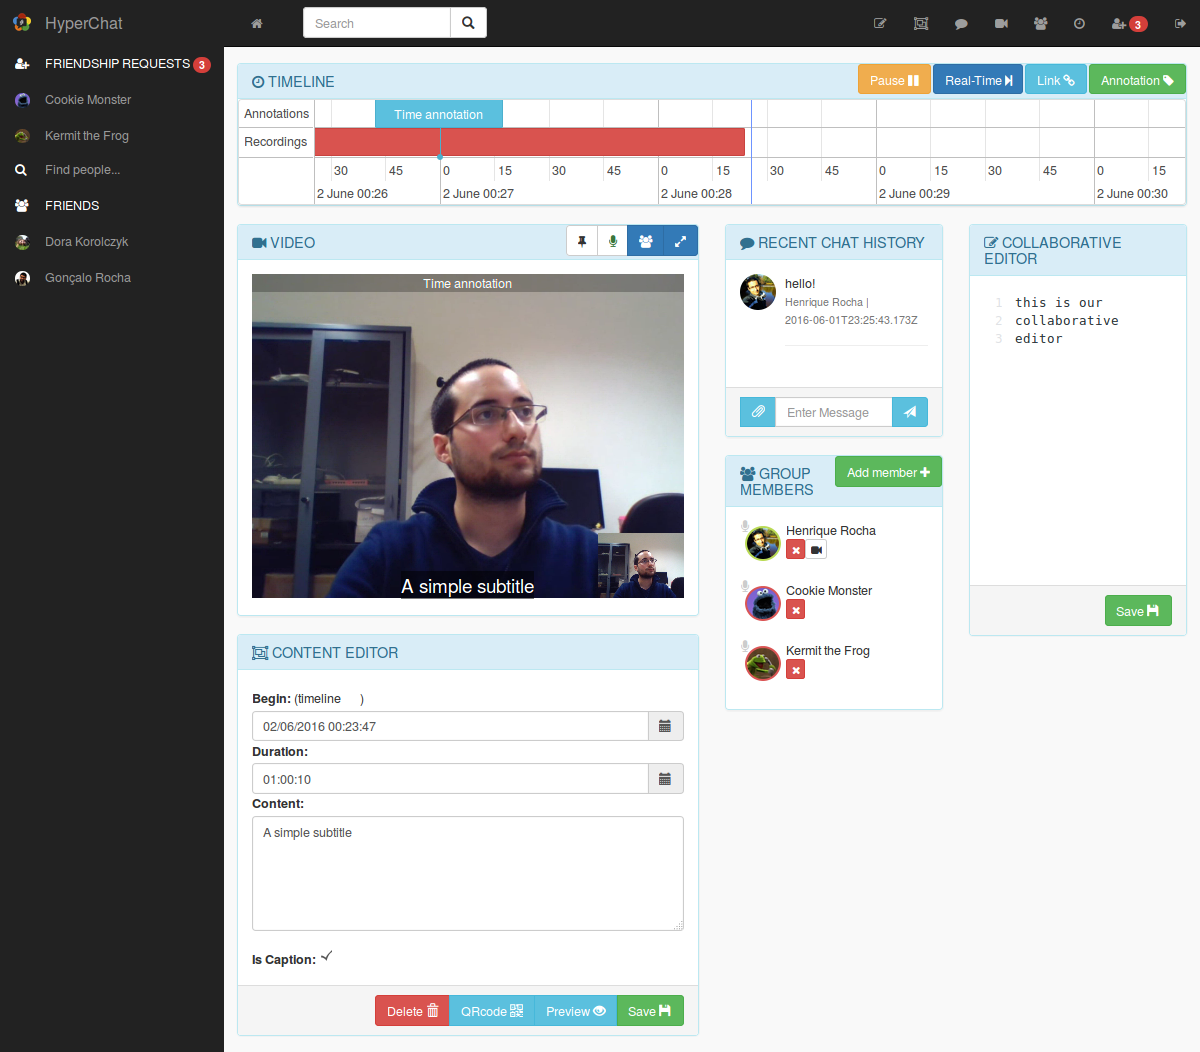
\includegraphics[width=0.8\textwidth]{figures/sshot.png}
		\end{center}
		\end{frame}



\section{Evaluation}\label{arch}

%\begin{frame}[t,shrink]
%\frametitle{Evaluation} 
%\tableofcontents[currentsection,hideothersubsections]
%\end{frame}

\subsection{Performance Tests}

	\begin{frame}[c]
		\frametitle{Performance Tests at Server - CPU Usage}
		\begin{figure}[H]
			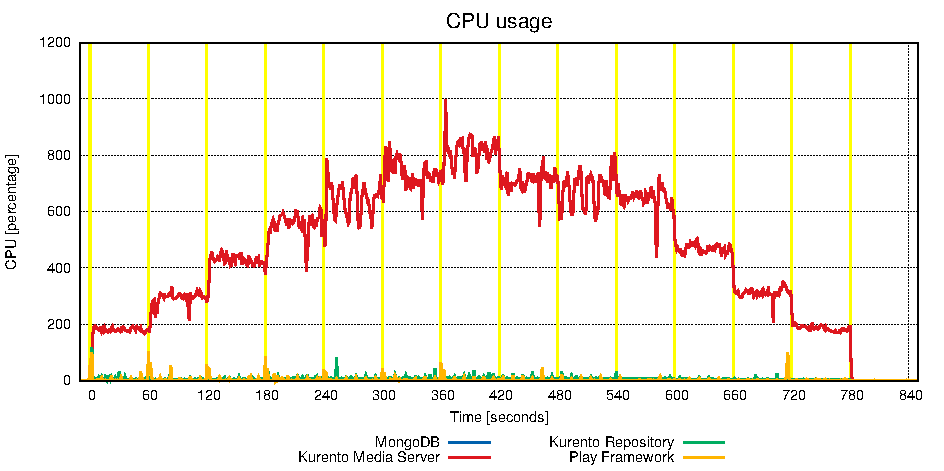
\includegraphics[width=\textwidth]{figures/cpu.pdf}
		\end{figure}
	\end{frame}
	\begin{frame}[c]
		\frametitle{Performance Tests at Server - Memory Usage}
		\begin{figure}[H]
			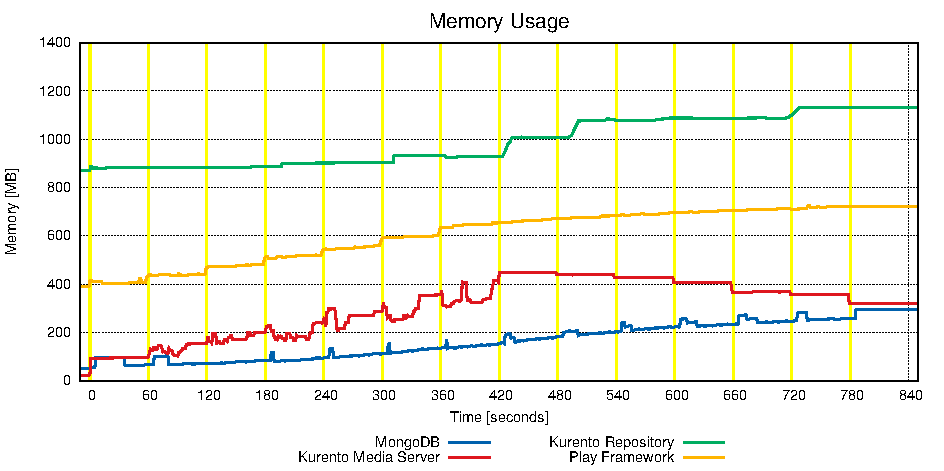
\includegraphics[width=\textwidth]{figures/ram.pdf}
		\end{figure}
	\end{frame}
	\begin{frame}[c]
		\frametitle{Performance Tests at Server - Network Usage}
		\begin{figure}[H]
			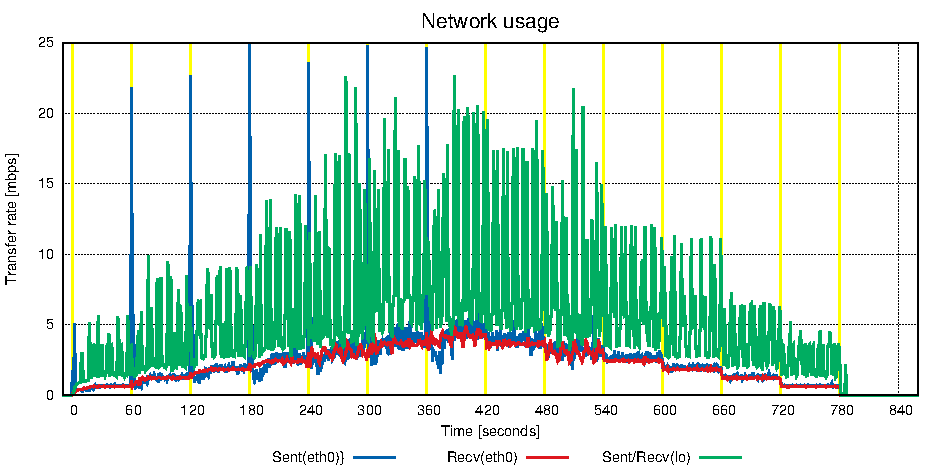
\includegraphics[width=\textwidth]{figures/net.pdf}
		\end{figure}
	\end{frame}

	\begin{frame}[c]
		\frametitle{Performance Tests at Client - Network Usage}
		\begin{figure}[H]
			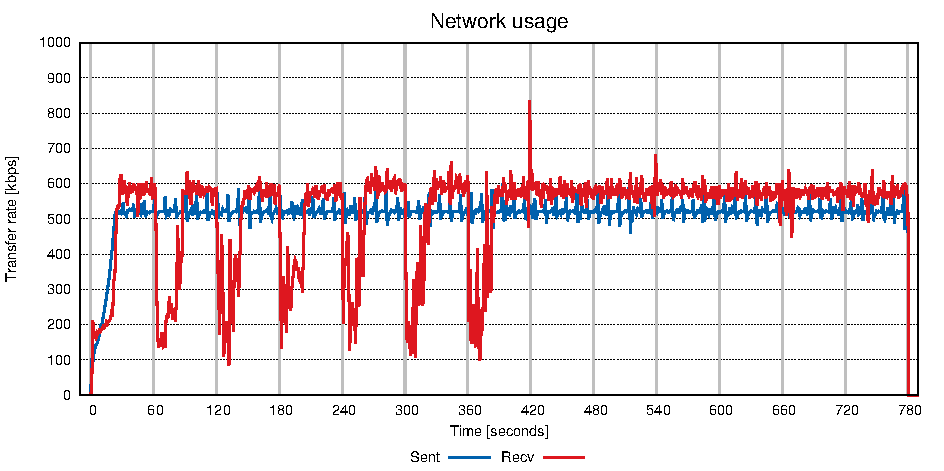
\includegraphics[width=\textwidth]{figures/net_clt.pdf}
		\end{figure}
	\end{frame}

\subsection{User Interface Tests}

	\begin{frame}[c]
		\frametitle{Usability tests}
		\begin{figure}[H]
			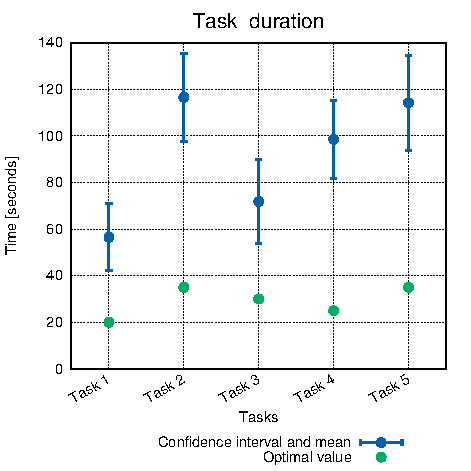
\includegraphics[width=0.5\textwidth]{figures/user_times.pdf}
			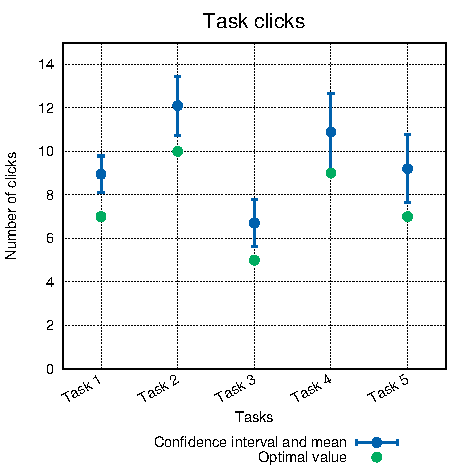
\includegraphics[width=0.5\textwidth]{figures/user_clicks.pdf}
		\end{figure}
		\begin{itemize}
			\item Difficulty per task.
			\item Errors per task.
		\end{itemize}
	\end{frame}
	\begin{frame}[c]
		\frametitle{Overall evaluation}
		\begin{figure}[H]
			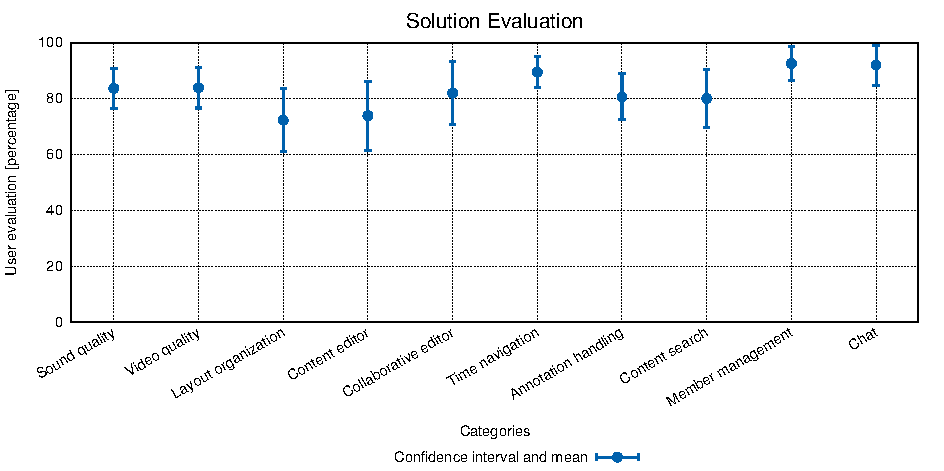
\includegraphics[width=\textwidth]{figures/user_evals.pdf}
		\end{figure}
	\end{frame}

\section{Conclusions}\label{concl} % English
%\begin{frame}[t,shrink]
%\frametitle{Related Work} 
%\tableofcontents[currentsection,hideothersubsections]
%\end{frame}

\begin{frame}[c]
		\frametitle{Conclusions}
		\begin{itemize}
\item New usage scenarios for communication and collaboration applications.
		\vfill

\item Enrich communications using hypermedia concepts. Record, playback and collaboration features.
		\vfill

\item Prototype implementation and testing.
		\end{itemize}

	\end{frame}


\section{Future Work}\label{concl} % English
%\begin{frame}[t,shrink]
%\frametitle{Related Work} 
%\tableofcontents[currentsection,hideothersubsections]
%\end{frame}

\begin{frame}[c]
		\frametitle{Future Work}
		\begin{itemize}
\item Implement fast-forward playback.
		\vfill

\item Improve solution's security.
		\vfill

\item Scale our solution to multiple servers.
		\end{itemize}

	\end{frame}



%------------------------------------------------

%------------------------------------------------

%------------------------------------------------

\begin{frame}[c]
\Huge{\centerline{Questions?}}
\end{frame}
	\begin{frame}[c]
		\frametitle{Performance Tests - CPU (average)}
		\begin{figure}[H]
			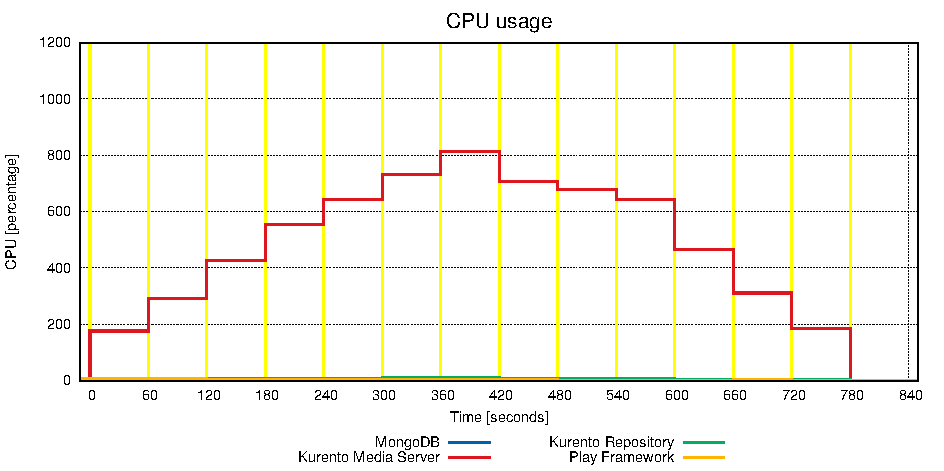
\includegraphics[width=\textwidth]{figures/cpu_avg.pdf}
		\end{figure}
	\end{frame}

	\begin{frame}[c]
		\frametitle{Performance Tests - Network Usage (average)}
		\begin{figure}[H]
			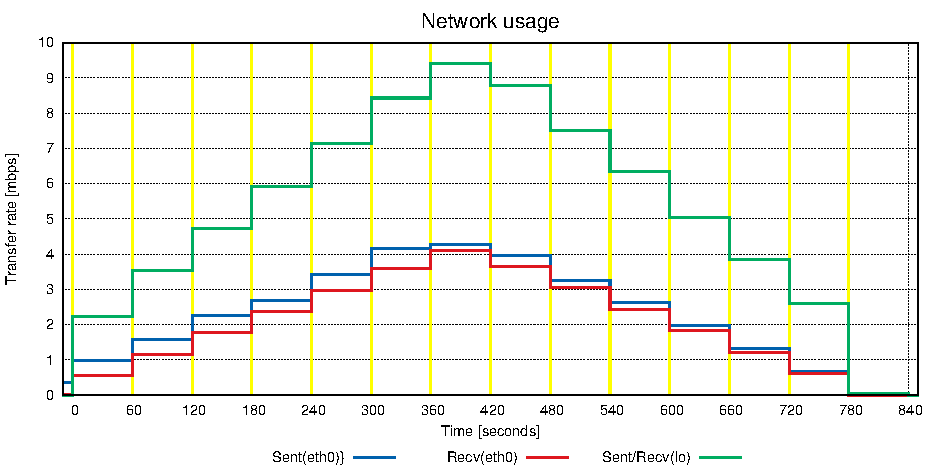
\includegraphics[width=\textwidth]{figures/net_avg.pdf}
		\end{figure}
	\end{frame}


	\begin{frame}[c]
		\frametitle{User Interface Tests}
		\begin{figure}[H]
			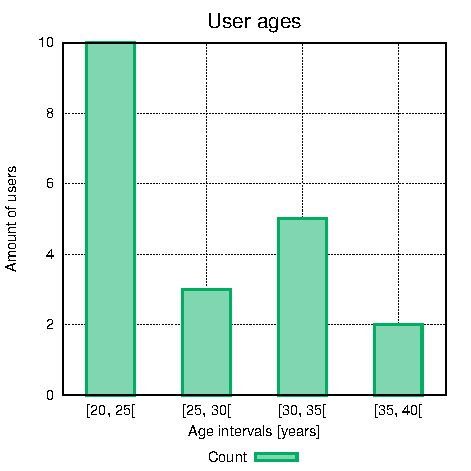
\includegraphics[width=0.5\textwidth]{figures/user_ages.pdf}
		\end{figure}
	\end{frame}

	\begin{frame}[c]
		\frametitle{Five tasks}
		\begin{figure}[H]
			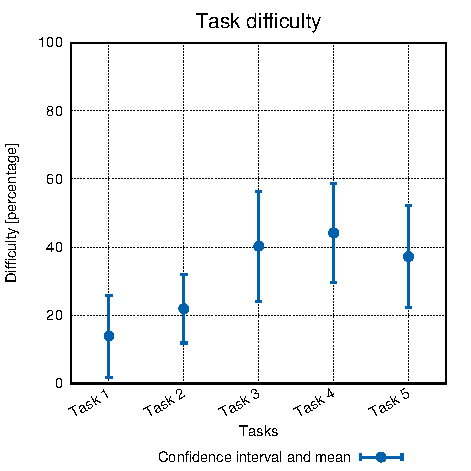
\includegraphics[width=0.5\textwidth]{figures/user_diffs.pdf}
			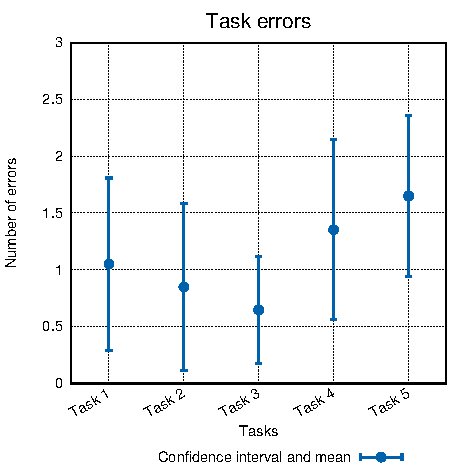
\includegraphics[width=0.5\textwidth]{figures/user_errors.pdf}
		\end{figure}
	\end{frame}

	\begin{frame}[c]
		\frametitle{Web Browser support}
		\Wider{
\begin{table}
			\label{table:otcomparision}
			\begin{tabular}{lr}
			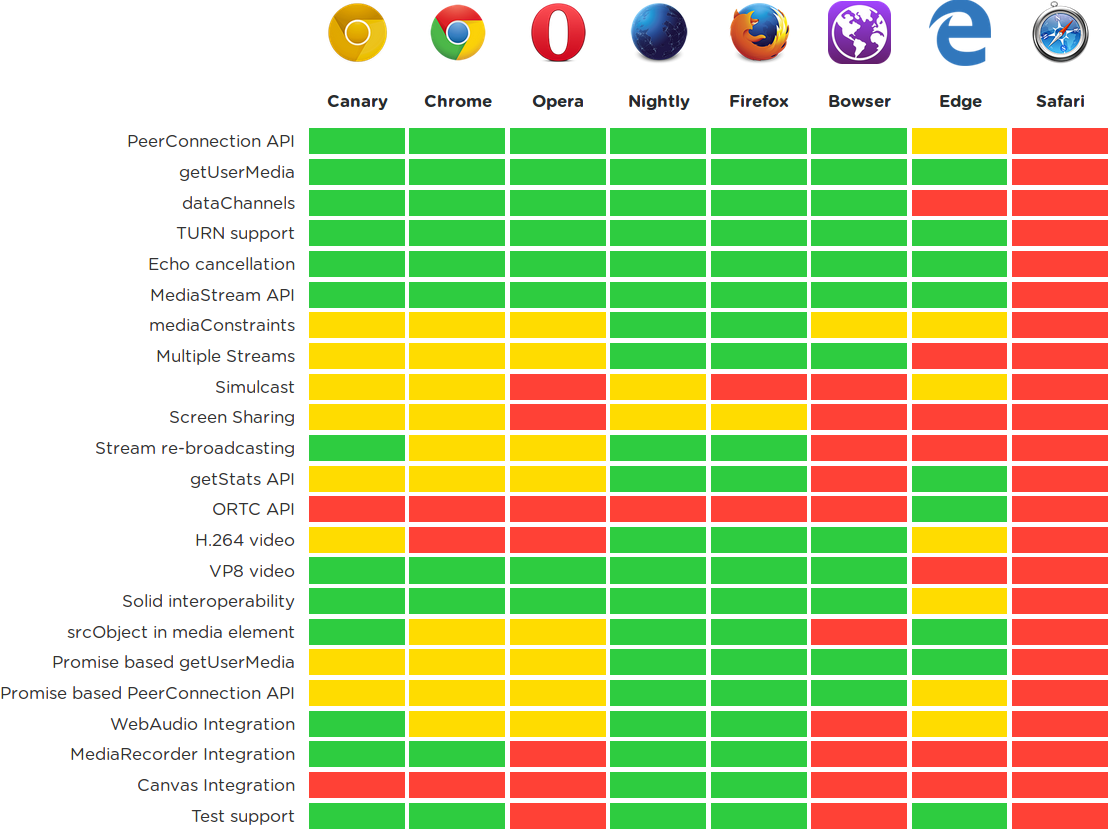
\includegraphics[width=0.8\textwidth]{figures/ready.png} & 	
\includegraphics[width=0.2\textwidth]{figures/space.png}

			\end{tabular}
			\end{table}}

		
	\end{frame}

	\begin{frame}[c]
		\frametitle{Security Concerns}
		\begin{itemize}
		\item Subset of actions implemented and triggered by messages. 
				\vfill
		\item Defined actions on demand, requires detecting malicious code.
		\begin{itemize}
			\item EarlyBird - machine learning techniques.
		\end{itemize}
	\end{itemize}

	\end{frame}

	\begin{frame}[c]
		\frametitle{Scalability}
		\begin{itemize}
				\vfill
		\item Kurento Media Server and \\ Kurento Repository in \\the same machine. 
				\vfill
		\item Fast data transfer on \\ localhost.
				\vfill
		\item Database bottleneck
		\end{itemize}

		\begin{flushright}
			\vspace*{-12\baselineskip}
			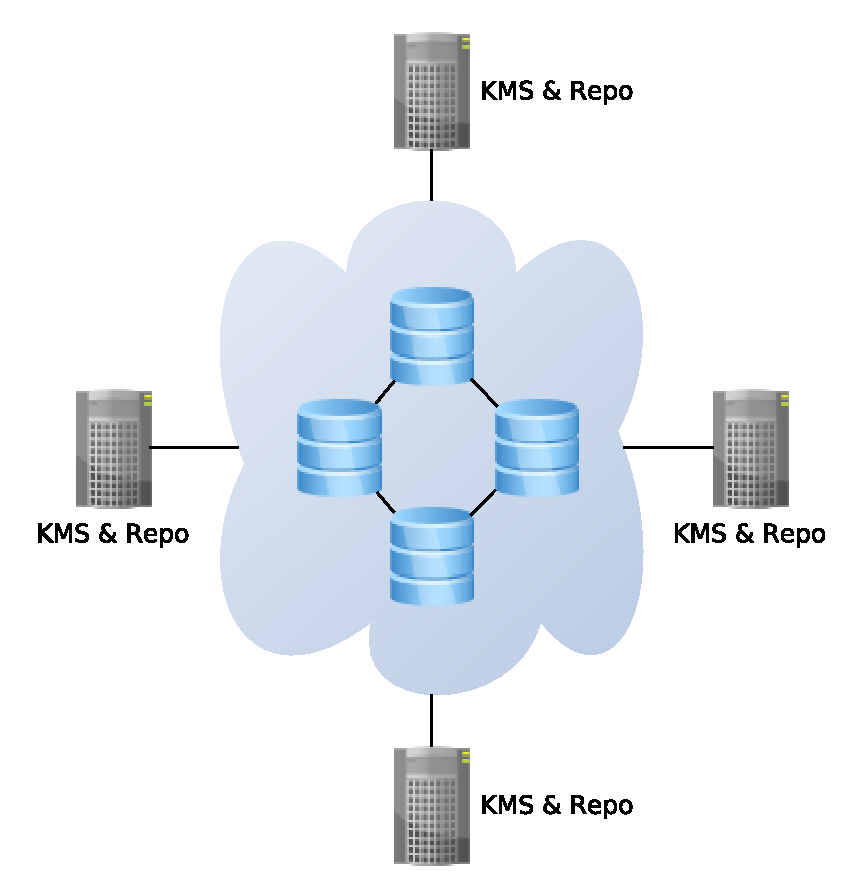
\includegraphics[width=0.5\textwidth]{figures/scale2.pdf}
		\end{flushright}
	


	\end{frame}

	\begin{frame}[c]
		\frametitle{Fast Forward}
		\begin{itemize}
				\vfill
		\item Implement fast forward on Kurento Media Server.
				\vfill
		\item Convert videos in real time with a new playback velocity using \emph{ffmpeg}.
				\vfill
		\item Convert videos after recording with predefined playback velocities.
		\end{itemize}


	\end{frame}

	\begin{frame}[c]
		\frametitle{Memory Usage}

		\begin{itemize}
				\vfill
				\item MongoDB - Always receiving data, caches inserted data on RAM. Checkpoints data to disk every 60 seconds or when journal data exceeds
2GB.
				\vfill 
				\item Play Framework - JVM uses memory recycling techniques instead of releasing to operating system.
				\vfill
				\item Kurento Repository - Caching videos.
				\vfill
				\item Kurento Media Server - Releases some memory and also recycles some of it.

		\end{itemize}
	\end{frame}

%----------------------------------------------------------------------------------------

\end{document} 
